%%%%%%%%%%%%%%%%%%%%%%%%%%%%%%%%%%%%%%%%%
% Journal Article
% LaTeX Template
% Version 1.4 (15/5/16)
%
% This template has been downloaded from:
% http://www.LaTeXTemplates.com
%
% Original author:
% Frits Wenneker (http://www.howtotex.com) with extensive modifications by
% Vel (vel@LaTeXTemplates.com)
%
% License:
% CC BY-NC-SA 3.0 (http://creativecommons.org/licenses/by-nc-sa/3.0/)
%
%%%%%%%%%%%%%%%%%%%%%%%%%%%%%%%%%%%%%%%%%

%----------------------------------------------------------------------------------------
%	PACKAGES AND OTHER DOCUMENT CONFIGURATIONS
%----------------------------------------------------------------------------------------

\documentclass[twoside,twocolumn]{article}

\usepackage[utf8]{inputenc}
\usepackage[T1]{fontenc}

\usepackage{blindtext} % Package to generate dummy text throughout this template

\usepackage[sc]{mathpazo} % Use the Palatino font
\usepackage[T1]{fontenc} % Use 8-bit encoding that has 256 glyphs
\linespread{1.05} % Line spacing - Palatino needs more space between lines
\usepackage{microtype} % Slightly tweak font spacing for aesthetics

\usepackage[english]{babel} % Language hyphenation and typographical rules

\usepackage[hmarginratio=1:1,top=32mm,columnsep=20pt]{geometry} % Document margins
\usepackage[hang, small,labelfont=bf,up,textfont=it,up]{caption} % Custom captions under/above floats in tables or figures
\usepackage{booktabs} % Horizontal rules in tables

\usepackage{lettrine} % The lettrine is the first enlarged letter at the beginning of the text

\usepackage{enumitem} % Customized lists
\setlist[itemize]{noitemsep} % Make itemize lists more compact

\usepackage{abstract} % Allows abstract customization
\renewcommand{\abstractnamefont}{\normalfont\bfseries} % Set the "Abstract" text to bold
\renewcommand{\abstracttextfont}{\normalfont\small\itshape} % Set the abstract itself to small italic text

\usepackage{titlesec} % Allows customization of titles
\renewcommand\thesection{\Roman{section}} % Roman numerals for the sections
\renewcommand\thesubsection{\roman{subsection}} % roman numerals for subsections
\titleformat{\section}[block]{\large\scshape\centering}{\thesection.}{1em}{} % Change the look of the section titles
\titleformat{\subsection}[block]{\large}{\thesubsection.}{1em}{} % Change the look of the section titles

\usepackage{fancyhdr} % Headers and footers
\pagestyle{fancy} % All pages have headers and footers
\fancyhead{} % Blank out the default header
\fancyfoot{} % Blank out the default footer
\fancyhead[C]{Affiliation Recommendation using Auxiliary Networks $\bullet$ Feb 2018} % Custom header text
\fancyfoot[RO,LE]{\thepage} % Custom footer text

\usepackage{titling} % Customizing the title section

\usepackage{hyperref} % For hyperlinks in the PDF

\usepackage{amsmath}
\usepackage{graphicx}

%----------------------------------------------------------------------------------------
%	TITLE SECTION
%----------------------------------------------------------------------------------------

\setlength{\droptitle}{-4\baselineskip} % Move the title up

\pretitle{\begin{center}\Huge\bfseries} % Article title formatting
\posttitle{\end{center}} % Article title closing formatting
\title{Affiliation Recommendation using Auxiliary Networks} % Article title
\author{%
\textsc{Petra Brčić, Ivan Čeh, Sandro Lovnički}\\[1ex]%\thanks{A thank you or further information} % Your name
\normalsize University of Zagreb, Faculty of Science, Department of Mathematics \\ % Your institution
%\normalsize \href{mailto:john@smith.com}{john@smith.com} % Your email address
%\and % Uncomment if 2 authors are required, duplicate these 4 lines if more
%\textsc{Jane Smith}\thanks{Corresponding author} \\[1ex] % Second author's name
%\normalsize University of Utah \\ % Second author's institution
%\normalsize \href{mailto:jane@smith.com}{jane@smith.com} % Second author's email address
}
\date{\today} % Leave empty to omit a date
\renewcommand{\maketitlehookd}{%
\begin{abstract}
\noindent Many social networks today, beside friendships, contain various groups and communities users associate with. Therefore, we can distinguish many co-existent structures within given network, such as user-to-user and user-to-group connections. The goal of this work is to calculate group affiliation recomendation for each user. Implications of those calculations span beyond social networks and can be applied to a wide range of problems.  % Dummy abstract text - replace \blindtext with your abstract text
\end{abstract}
}

%----------------------------------------------------------------------------------------

\begin{document}

% Print the title
\maketitle

%----------------------------------------------------------------------------------------
%	ARTICLE CONTENTS
%----------------------------------------------------------------------------------------

\section{Introduction}

Predicting the future state of social networks has become a major occupation of scientists in recent years, thus data science as a discipline is growing more rapidly each day. Furthermore, there is a lot of interest in affiliation recomendation in today's over more competitive market. Nonetheless, approaches mentioned in this paper can even be extended to a vairety of non-social problems such as the problem of identifying genes affecting certain traits from observed genes-to-genes and genes-to-traits connections.

{\large\textit{Our network.}} Today's social networks have a lot of restrictions on their public API as well as strict laws against content crawling, so we decided to build our own social network of virtual users and groups. It is composed of users and groups, each having their capabilities which will be briefly described here and can, together with models calculations, be closely observed in our \href{https://github.com/Qkvad/AffiliationRecommendation}{GitHub repository}. Our network is created in distinct steps; groups creation, users creation, groups initial population, users be-friending. Last step is the most interesting one. User adds number of friends from list of all friends dependant on its popularity. There exist 1\% of "super-popular" users who are at least 2 times more popular than regular users. Friendship is symetrical, that is, when an user adds new friend, this friend also adds him. This can easily be changed to be non-symetrical. Users, execpt their initial group membersihps also decide to join groups which their friends are members of and tthey do that 25\% of the time.\\
Method described above yields a very good and "real-structured" social-network from which existant user connections and group affiliations are easily extracted in the form of later mentioned matrices A and S.

%------------------------------------------------

\section{Models}
In this section, we will establish the notation used in models that follow. \\
Notation. Let the $N_u$ be the number of users and $N_g$ be the number of groups. We define matrix $A \in \mathbb{R}^{N_u \times N_g}$ which denotes user$\times$group matrix or adjacency matrix of affiliation network and matrix $S \in \mathbb{R}^{N_u \times N_u}$ which denotes user$\times$user matrix or adjacency matrix of friendship. \\

The task is to recommend affiliations to a given user, we tackeled all the users simultaniously. The problem can be posed as a problem of ranking affilations in order of the users interest in joining them. Methods that will be introduced later solve the problem by assigning scores to various affiliations in order to rank them. \\

Consider the adjacency matrices $A$ and $S$. We assume $S$ is symmetric, if user $i$ is friend to user $j$ then user $j$ is friend to user $i$. Matrix $S$ corresponds to undirected graph among users and $\begin{bmatrix} 	0 & A\\ 	A^T & 0 \end{bmatrix}$ corresponds to undirected bipartite graph between users and groups. We will also define a graph $C$ between all users and groups, with the combined adjacency matrix  $ C= \begin{bmatrix} 	\lambda S & A\\ 	A^T & 0 \end{bmatrix}$. Parametar $\lambda$ controls the ratio of the weight of friendship to the weight of group membership. If $\lambda = 0$ we have bipartite affiliations graph. \\

Models we are introducing are Graph proximity model and Latent factors model to calculate score matrices.



\subsection{Graph proximity model}
We start by assuming that the graph is known and the prediction of new links between nodes is going to be examined by calculating proximity. As we mentioned, the affiliation network can be modeled by a graph, so the basic idea is that there is possible link between two nodes based on the proximity between them. Proximity can be calculated as sum of number of paths  that connect them, paths of different lengths. \\
We are going to use Katz measure for calculating proximity. Katz measure is used to measure the relative degree of influence of a node in a network.
\[ Katz(S;\beta) = \sum_{n=1}^{\infty} \beta^n S^n = \beta S +\beta^2 S^2 + \beta^3 S^3 + ...  \]
We extend the Katz measure to the bipartitie graph A
\[ Katz(A;\beta) = \beta A A^T A +\beta^2 (AA^T)^2 A + ...  \]
where in the co-occurence matrix $A A^T$, two users $i$ and $j$ are considered connected if $i$ and $j$ belong to at least one same group, i.e. $(AA^T)_{i,j} > 0$. We consider paths from user $i$ to user $j$ by $AA^T$, and then user $j$ to some other user $k$ by $AA^T$ and then user $k$ to some group by $A$. Idea is that if user $i$ shares some community with $j$ it is more likely $i$ will join some community $j$ belongs to. \\
We will now expand Katz measure on the combined graph $C$
\[ Katz(C;\beta) = \beta C +\beta^2 C^2 + ...  \]
\[ Katz(C;\beta) = \beta A +\beta^2 \lambda S A +  \beta^3( \lambda^2 S^2A + A A^T A ) + ...  \]
This Katz measure generalizes the normal Katz measure by also considering some paths from user $i$ to user $j$ by matrix $S$, then user $j$ to some group by matrix $A$. And also user $i$ to user $j$ by $S$, user $j$ to user $k$ by $AA^T$ then again user $k$ to user $j$ by $A$ and finaly user $j$ to some group by $A$. The matrix given by $Katz(C;\beta)$ can be used as score matrix.
In case of higher dimension of matrices you work with, truncated Katz is preffered, but for our problems we stick to normal Katz because matrices for testing are not high dimensional. \\
We will just roughly discuss which $\beta$ and $\lambda$ we should take. In our algorithms $\beta$ is calculated as reciprocal of the maximum absolute value of eigenvalues of matrix $A$. Usually we take $\lambda = 0.2$ but the point of that parametar is to factor the significance of user to user matrix and the connections between users itself.

\subsection{Latent factors model}

In Latent factors model we start with matrices $A$ and $S$ defined same as before. We use them to form the matrix
$ C^\prime (\lambda, D) = \begin{bmatrix} \lambda S & A\\ A^T & D \end{bmatrix} $. \\
Zeros in $A$ and $S$ are viewed as unobserved entries with high probability of being zero. $D$ is the derived similarity between groups. Often $A^TA$ or $\lambda A^TA$ are used as $D$. \\
We assume $A \approx U^T G$ where $U \in \mathbb{R}^{d \times N_u}$, $G \in \mathbb{R}^{d \times N_g}$ where $d \ll N_u, N_g$. With fixed value of $d$ we want $C^\prime (\lambda, D) \approx \begin{bmatrix} U^T\\ G^T \end{bmatrix}\begin{bmatrix}U&G \end{bmatrix}$ in terms of Frobenius norm. \\
Solution of this problem is given by SVD decomposition of $C^\prime$: $C^\prime \approx U \Sigma G^T$ where $U$ is the matrix of $d$ leading singular vectors, $\Sigma$ is $d \times d$ matrix of $d$ highest singular values and $G$ is the matrix of $d$ leading singular vectors. We can interpret this approximation as the score matrix.

%------------------------------------------------

\section{Discussion}

We tested our calculations on a variety of different networks, ranging from large to small, from containing extremely popular users or groups to having equally spread popularity.

%%%%%%%%%% users_graph

\begin{figure}[h]
	\centering
	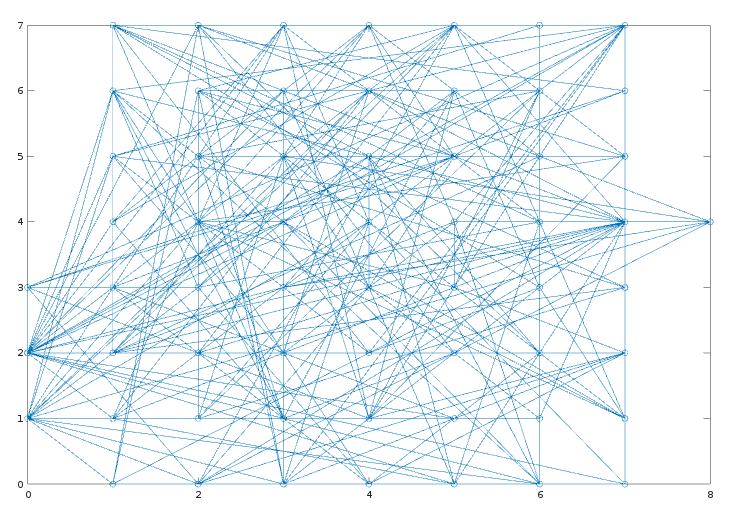
\includegraphics[width=0.5\textwidth]{users_graph}
	\caption{Graph of $user \times user$}
	\label{pic1}
\end{figure}

\subsection{Results}

Results obtained by 2 different models (graph proximity and latent factors) agree on suprisingly large number of suggestions: cases in which they do not agree in any of $c$ suggestions for a specific user are extremely rare and occur in less than $1\%$ of the time.

%%%%%%%%% latent_katzC-sim

\begin{figure}[h]
	\centering
	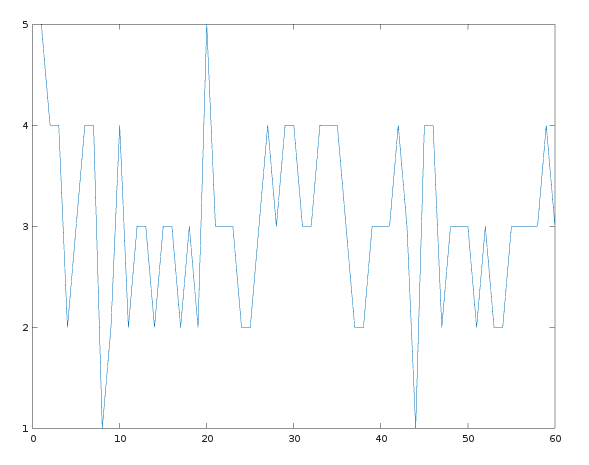
\includegraphics[width=0.5\textwidth]{latent_katzC_sim}
	\caption{Number of the same top 5 recommendations obtained with Graph proximity model and Latent factors model}
	\label{pic1}
\end{figure}

%----------------------------------------------------------------------------------------
%	REFERENCE LIST
%----------------------------------------------------------------------------------------
\pagebreak
\begin{thebibliography}{99} % Bibliography - this is intentionally simple in this template

\bibitem[1]{AffRec}
Vishvas Vasuki, Zhengdong Lu, Nagarajan Natarajan, Inderjit Dhillon.
\newblock Affiliation Recommendation using Auxiliary Networks.

\bibitem[2]{MesMeth}
Alan Mislove, Massimiliano Marcon, Krishna P. Gummadi, Peter Druschel, Bobby Bhattacharjee.
\newblock Measurement and Analysis of Online Social Networks.



\end{thebibliography}

%----------------------------------------------------------------------------------------

\end{document}
